\documentclass{article}
\usepackage{graphicx}
\usepackage[utf8]{inputenc}
\usepackage[T1]{polski}
\usepackage{amsmath}
\graphicspath{ {res/} }
 
\begin{document}

\section{Błąd średniokwadratowy w funkcji ilości emiterów i detektorów.}
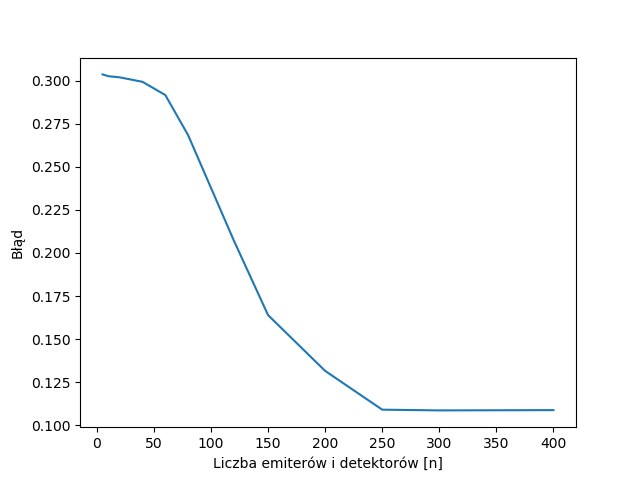
\includegraphics[width=\textwidth]{wykres}
\centering

\section{Błąd średniokwadratowy w zależności od zastosowanych filtrów.}
n=100
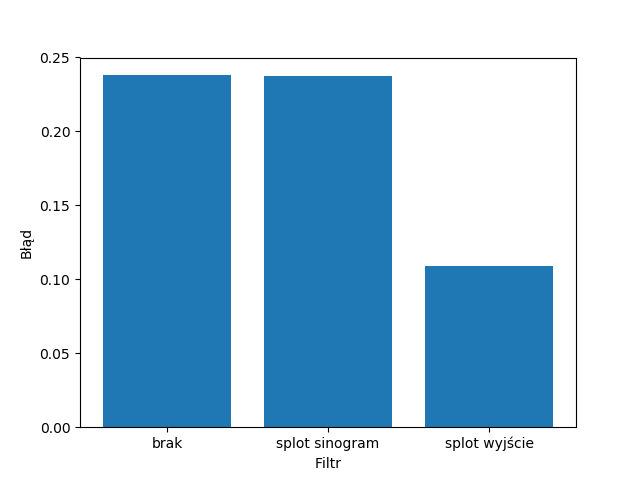
\includegraphics[width=\textwidth]{wykres2}
\centering
 
\end{document}